 \documentclass[main]{subfiles}

\begin{document}
\chapter{Marco Metodológico.}

La investigación realizada se clasifica según su objeto como correlacional ya que mide el grado de relación entre la cinemática de los ejes respecto a las cargas en la interacción rueda riel. Así mismo se trata de una investigación diacrónicas ya que compará los resultados obtenidos por Metro de Caracas C.A. en 2001 y se compara los resultados obtenidos en el 2011.

\section{Diseño de la investigación.}
El estudio realizado en esta investigación sigue un diseño no experimental, de tipo transversal correlacional, ya que, como se mencionó en el tipo de investigación se compara la cinemática de los ejes respecto a las cargas en la interacción rueda riel, sin embargo las variables de fuga no es controlada sino se que recopilaron a lo largo de una serie de mediciones realizadas en segmentos de vía a lo largo de la línea 1.

\section{Muestra del Estudio.}

Se recopilaron una serie de mediciones a lo largo de la línea 1 de Metro de Caracas, registrando las cargas longitudinales, laterales y verticales, y los movimientos del eje durante su recorrido.  Además se realizaron mediciones de la rugosidad de los rieles para estimar los valores de coeficiente de roce.

La data recopilada en 2001 comprendio de XX de las 12 estaciones que forman en conjunto la línea 1 de Metro de Caracas C.A. Se analizó un muestreo de XX de esos elementos para establecer la relación entre las deformaciones registradas por Metro de Caracas en la superficie de la rueda con la relación a las cargas en el punto de contacto.

Cuando se estableció un modelo para la relación de las deformaciones en la rueda con las cargas tangenciales y normales a la misma, se tomaron muestras de NN estaciones por cada día de prueba, seleccionados de manera aleatoria.

\section{Técnicas e instrumentos de recolección de datos.}

La investigación se realiza en dos etapas, la primera etapa consistió en establecer la metodología para la obtención de las cargas en el contacto rueda riel. Mientras que una segunda etapa consistió en la recopilación de datos y análisis de los mismos.

Para la recopilación de datos, se utilizó un equipo denominado ejes instrumentados que consiste en un conjunto de dos ejes cuyas ruedas incorporan una serie de galgas extensiometricas ubicada en la superficie interna de la rueda. Las deformaciones registradas permiten de manera empírica establecer las distintas cargas aplicadas y la ubicación donde ocurre el contacto mecánico.


\begin{figure}[!htbp]
\centering
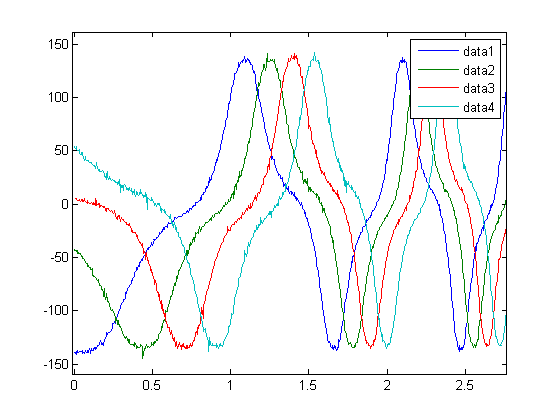
\includegraphics[scale=0.7]{DataGraf.png}
  \caption{Resultados de las deformaciones verticales obtenidas por Metro de Caracas en 2001}
  \label{fig:DataGraf}
\end{figure}  

La relación entre las deformaciones y las cargas aplicadas se logró obtener mediante regresiones múltiples a partir de los datos registrados en el 2001. Estas deformaciones, tal como se muestra el figura \ref{fig:DataGraf} describen un comportamiento sinusoidal debido al puente de wheatstone que cambia la polaridad de la señal cada 90º. Además la variación en la frecuencia de la señal se debe a la variación de la velocidad angular presente en la rueda, escenario que se observa principalmente en los arranques y frenados del tren.

Dado el comportamiento de las señales fue necesario establecer un modelo que pudiese establecer la relación entre carga y deformación. Para ello se propuso un modelo lineal basado en la sumatoria del valor absoluto de cada señal multiplicando por una constante cuyo valor fue obtenido mediante regresión múltiple.

\begin{equation}
F(\varepsilon_{zij})=\sum A_{i,j} \cdot \varepsilon_{ij}
\end{equation}

\section{Técnicas de análisis de los datos.}

La base objetiva en la que se fundamenta este trabajo, es la determinación de la calidad del contacto rueda riel presente en las dos superficies. Esta calidad por tanto se define como la aproximación a las condiciones ideales de los fenómenos presentes en el contacto.

Para determinar las condiciones que conlleva a una buena calidad del contacto rueda se estableció una serie de criterios basados en la naturaleza de las variables que participan en ella. Los fenómenos de estudio que pueden ser evaluados directamente en función de las variables presentes y medibles fueron definidos como criterios exógenos, en cambio los fenómenos que las variables de estudios solo permiten comparar un patrón ideal respecto a la respuesta medible son definidos como endógenos.

Los criterios exógenos, se apegan principalmente a las normas internacionales ferroviarias, en este caso la norma UIC518 que establece patrones de comportamiento no deseado. Adicionalmente se incluyeron las condiciones donde el punto de contacto rueda riel, se lleva a cabo en zonas puntos del perfil de la rueda que comprometen la estabilidad del sistema.

%Descripción

Los criterios endógenos se definieron por el área de contacto ideal y real del contacto mecánico. Mediante el modelo de distribución de presión normal, es posible estimar el área de contacto ideal y mediante el modelo de distribución lineal de presión tangencial de Kalker para establecer la carga tangencial. La diferencia entre las dos cargas, implica que las condiciones del contacto varían en cierta medida serán observadas desde el espectro de las variables de los modelos de contacto rueda riel. 

Inicialmente se establece discretación del contacto rueda riel la ubicación del punto de contacto. Se segmenta el perfil en tramos cuyas características geométricas son constantes a lo largo de cada segmento, el perfil aproximado se puede observar en la figura NN al igual que en la segmentación del perfil. En la siguiente tabla, se describen las características geométricas para cada segmento:
\newline

\begin{figure}[!htbp]
\centering
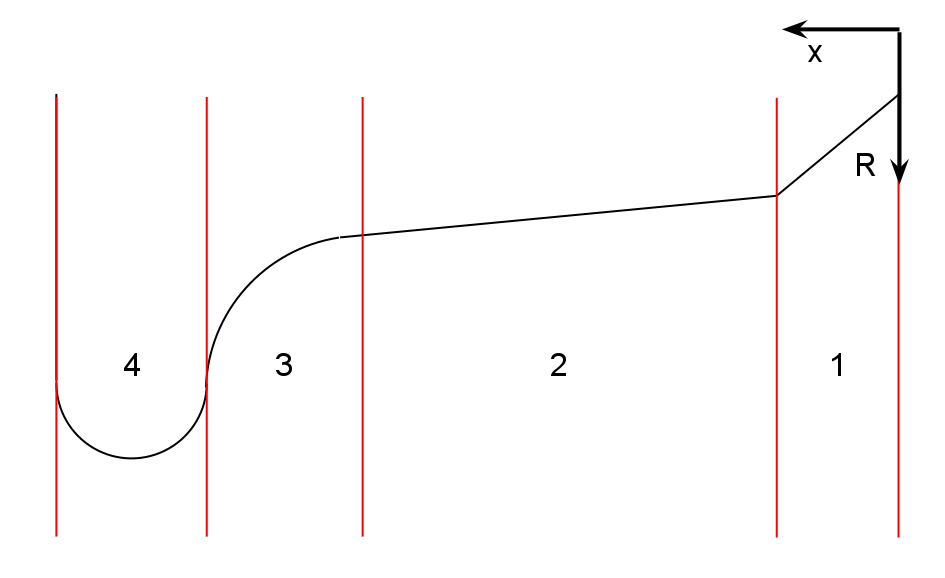
\includegraphics[scale=0.3]{WheelProf.png}
  \caption{Perfil de la rueda divida en segmentos, la el dibujo es figurativo y la descripción de los segmentos se encuentra en la tabla.}
  \label{fig:DataGraf}
\end{figure}  

\begin{center}
\begin{table}[!htbp]
\caption{Descripción de los segmentos de acuerdo al punto de contacto.}
\begin{tabular}{|c|c|c|c|c|c|c|c|}
\hline
Seg:& $X_o$ & $X_f$ &  $\gamma$ & $Rx_w$ & $Ry_w$ & $Rx_r$ & $Ry_r$ \\
\hline
1& $0$ & $30$ & $0.15$ & $413.75 \rightarrow 418.25$  & $0$ & $0$ & $250$ \\
\hline
2& $30$ & $82$ &  $0.05$ & $418.25 \rightarrow 420.845$  & $0$ & $0$ & $250$  \\
\hline
3& $82$ & $105$ &  $\frac{x-80.69}{\sqrt{691.69-(x-80.69)^2}}$ & $\frac{\sqrt{691.69-(x-80.69)^2}+447.11}{cos(\gamma)}$ &   $-26.30$ & $0$ & $Ry_r$ \\
\hline
4& $105$ & $135$ &  $\frac{x-118.33}{\sqrt{277.89-(x-118.33)^2}}$ & $\frac{\sqrt{277.89-(x-118.33)^2}+430.00}{cos(\gamma)}$ &   $16.63$ & $0$ & $250$ \\
\hline
\end{tabular}
\end{table}
\end{center}


Debido a la conicidad de la rueda, es necesario descomponer la componente de la carga que interactúa en la superficie de la rueda de manera perpendicular. La carga tangencial y normal, permiten por lo tanto definir la carga normal aplicada al riel y definir el área de contacto ideal. Las cargas verticales y laterales en la rueda, el sistema de coordenadas cartesianas se define como:

\begin{equation}
Q=N\{ cos(\gamma) + sin(\gamma) \cdot f_y \}
\end{equation}
\begin{equation}
Y=N\{ -sin(\gamma) + cos(\gamma) \cdot f_y \}
\end{equation} 
 
\par \hspace{2cm}
\begin{minipage}{8cm}
\begin{spacing}{0.5}
Donde:
\begin{itemize}
\item $Q$ es la carga vertical aplicada en el punto de contacto.
\item $Y$ es la carga lateral aplicada.
\item $\gamma$ la conicidad de la superficie en el punto de contacto.
\item $N$ la carga normal a la superficie.
\item $f_y$ la componente de la carga tangencial dada por la fuga.
\end{itemize}
\end{spacing}
\end{minipage}

Despejando la carga normal se obtiene:

\begin{equation}
N=Q\cdot cos(\gamma) - Y \cdot sin(\gamma) 
\end{equation}


La componente normal, permitirá definir el área de contacto ideal, en cuanto la componente tangencial, se descompondrá para determinar el área de contacto según la fuga presente. Para la determinación del área de contacto ideal, el modelo de contacto mecánico y distribución normal planteado por \citet{Herz1881} se maneja como referencia o punto de partida:

\begin{eqnarray}
r_m=\sqrt[3]{\frac{3\pi}{8}\frac{N(k_1+k_2)}{\beta}}
\\
a=m\cdot r_m
\\
b=n\cdot r_m
\end{eqnarray}

\par \hspace{2cm}
\begin{minipage}{8cm}
\begin{spacing}{0.5}
Donde:
\begin{itemize}
\item $k_1$ y $k_2$ Las constantes de elasticidad de Hertz.
\item $m$ y $n$ la proporción de los diametros de la elipse de contacto.
\item $a$ la mitad del diámetro de la elipse de contacto en la dirección de movimiento.
\item $b$ la mitad del diámetro de la elipse de contacto en la dirección perpendicular al movimiento.
\item $\beta$ constante definida por la gemetría del riel y la vía.
\end{itemize}
\end{spacing}
\end{minipage}

Definida el área de contacto, la estimación del deslizamiento lateral se definió por el concepto vectorial de fuga. Dentro de las limitaciones del problema de estudio, se estima que el fuga puede ser obtenida por el cambio de dirección del eje, no obstante una definición vectorial de fuga permite que, fuera del marco teórico contenido en este trabajo, se pueda estudiar el área de contacto en el arranque y frenado definido por \citet{Kalker1991243} como fenómeno de Catteneo. 

La definición vectorial de fuga viene dado por:


\begin{equation}
\{ \xi,\eta\}=\frac{\vec{V_w}-\vec{V}}{\|\vec{V}\|}
\end{equation}

\par \hspace{2cm}
\begin{minipage}{8cm}
\begin{spacing}{0.5}
Donde:
\begin{itemize}
\item $\vec{V_w}$: velocidad tangencial de la rueda.
\item $\vec{V}$: velocidad absoluta de la rueda.
\item $ \xi$: fuga longitudinal.
\item $\eta$: fuga lateral.
\end{itemize}
\end{spacing}
\end{minipage}

Por tanto la velocidad tangencial de la rueda es conocida en función de la velocidad angular de la rueda y la velocidad longitudinal mediante mediciones de aceleración en el boggie. La velocidad lateral se hará en función de la variación de la posición del punto de contacto por el tiempo. Igualmente se define que la dirección de la velocidad tangencial de la rueda y la velocidad real propia del cuerpo son iguales, ésta es una aproximación debido a las dificultades para determinar la fuga lateral.

La fuga lateral es definida como:

\begin{equation}
\eta=\frac{\vec{\omega}_w\cdot Rx'_w-\sqrt{\dot{y}^2+\dot{x}^2}}{\|\vec{V}\|}\cdot
\frac{\dot{y}}{\|\vec{V}\|} 
\end{equation}

\par \hspace{2cm}
\begin{minipage}{8cm}
\begin{spacing}{0.5}
Donde:
\begin{itemize}
\item $\vec{\omega_w}$: velocidad angular de la rueda.
\item $Rx'_w$: Radio de la rueda en el punto de contacto.
\item $\dot{x}$: velocidad longitudinal.
\item $\dot{y}$: velocidad lateral.
\end{itemize}
\end{spacing}
\end{minipage}

Una vez que se ha establecido la fuga lateral y el área ideal de contacto el problema reside en definir el área de contacto real de contacto. \citet{Kalker1991243} definió un coeficiente de rigidez de acuerdo al diámetro mayor y menor de la elipse de contacto ya definido por \citet{Herz1881}. Distintos modelos utilizan el coeficiente de Kalker como para la determinación de las cargas tangenciales. Desde este punto, el modelo lineal de cargas de Kalker, el modelo de heurístico de Shen et al y el modelo de Polach pueden ser utilizados para la determinación del área real de contacto. Los modelos basados en la estimación de la distribución de presión no son recomendados ya que requieren de un número de iteraciones considerable para estimaciones en tramos largos.

Para cualquiera de los tres métodos de contacto rueda riel, se estructuró una modificación de coeficientes de Kalker. El área de contacto mantiene un término constante que fue utilizado para simplificar los cambios geométricos en la vía. La determinación de los diámetros principales de la elipse de contacto radica en un radio primitivo, dependendiente de la carga aplicada y de la geometria del cuerpo presente en un escalar $m$ y $n$ definidos en la ecuación 1.6 y 1.7. Estos valores se determinan dada las curvaturas de los cuerpos en contacto:

\begin{equation}
	A+B=\frac{1}{Rx_w}+\frac{1}{Ry_w}+\frac{1}{Rx_r}+\frac{1}{Ry_r}
\end{equation}
\begin{equation}
	B-A=\frac{1}{2}
\sqrt{
\left( \frac{1}{Rx_w}-\frac{1}{Ry_w}\right) ^2
+\left( \frac{1}{Rx_w}-\frac{1}{Ry_w}\right) \cdot \left(\frac{1}{Rx_r}-\frac{1}{Ry_r}\right) 
+\left( \frac{1}{Rx_r}-\frac{1}{Ry_r}\right) ^2
}
\end{equation}

A+B y B-A es utilizado para determinar la relación entre el diametro mayor y menor de la elipse de contacto, por lo tanto m y n se definen como:

\begin{equation}
m(A,B)=f_1\left( arcos\left(\frac{B-A}{A+B} \right)\right)
\end{equation}
\begin{equation}
n(A,B)=f_2\left( arcos\left(\frac{B-A}{A+B} \right)\right)
\end{equation}

$f_1$ y $f_2$ fueron definidas por \citet{Herz1881} y se utilizaron para definir un nuevo coeficiente de rigidez geometrica, agrupando los valores que en si son constantes en los distintos modelos:

\begin{equation}
a\cdot b \cdot C_{ij}=r_m^2 \cdot m \cdot n \cdot C_{ij}
\end{equation}
Separando el término que depende de la carga:
\begin{equation}
Kr_{ij}= m \cdot n \cdot C_{ij}
\end{equation}
\newline
Para este trabajo, Kr fue computado obteniendo una tabla de valores de Kr para cada combinación:
\newline
{
\begin{spacing}{1} 

\begin{table}[!htbp]
\caption{Criterio de contacto geométrico para distintos valores de excentricidades y módulos de poisson, computados mediante octave.}
\small
\begin{tabular}{|c|c|c|c|c|c|c|c|c|c|c|}\hline
& \multicolumn{3}{|c|}{$ Kr_{11}$} &\multicolumn{3}{|c|}{$ Kr_{22}$} & \multicolumn{3}{|c|}{$ Kr_{23}$}\\ \hline 
$\Theta$& 0.0 & 0.25 & 0.5 &0.0 & 0.25 & 0.5 & 0.0 & 0.25 & 0.5\\ \hline
10 & 5,1417 & 6,8161 & 10,106 & 5,1417 & 5,1515 & 5,1613 & 0,3272 & 0,4634 & 0,7162\\ \hline
15 & 4,3974 & 5,8127 & 8,5629 & 4,3974 & 4,4108 & 4,4242 & 0,4474 & 0,6336 & 0,9792\\ \hline
20 & 3,9552 & 5,2101 & 7,6181 & 3,9552 & 3,9747 & 3,9929 & 0,5437 & 0,7598 & 1,1588\\ \hline
25 & 3,6709 & 4,8128 & 6,9729 & 3,6709 & 3,7039 & 3,7307 & 0,5740 & 0,7628 & 1,1029\\ \hline
30 & 3,4638 & 4,5184 & 6,4818 & 3,4638 & 3,5098 & 3,5449 & 0,6110 & 0,7774 & 1,0681\\ \hline
35 & 3,3174 & 4,3034 & 6,1118 & 3,3174 & 3,3766 & 3,4230 & 0,6484 & 0,7976 & 1,0506\\ \hline
40 & 3,2068 & 4,1351 & 5,8148 & 3,2068 & 3,2790 & 3,3391 & 0,6831 & 0,8189 & 1,0428\\ \hline
45 & 3,1335 & 4,0160 & 5,5870 & 3,1335 & 3,2197 & 3,2958 & 0,7240 & 0,8489 & 1,0481\\ \hline
50 & 3,0867 & 3,9339 & 5,4114 & 3,0867 & 3,1875 & 3,2844 & 0,7656 & 0,8834 & 1,0643\\ \hline
55 & 3,0593 & 3,8762 & 5,2670 & 3,0593 & 3,1753 & 3,2914 & 0,8108 & 0,9231 & 1,0883\\ \hline
60 & 3,0499 & 3,8402 & 5,1443 & 3,0499 & 3,1828 & 3,3157 & 0,8612 & 0,9701 & 1,1227\\ \hline
65 & 3,0653 & 3,8393 & 5,0942 & 3,0653 & 3,2172 & 3,3745 & 0,9197 & 1,0253 & 1,1776\\ \hline
70 & 3,0966 & 3,8535 & 5,0714 & 3,0966 & 3,2690 & 3,4516 & 0,9830 & 1,0885 & 1,2430\\ \hline
75 & 3,1461 & 3,8783 & 5,0571 & 3,1461 & 3,3405 & 3,5454 & 1,0513 & 1,1635 & 1,3161\\ \hline
80 & 3,2049 & 3,9302 & 5,0802 & 3,2049 & 3,4240 & 3,6624 & 1,1299 & 1,2499 & 1,4010\\ \hline
85 & 3,2849 & 4,0061 & 5,1209 & 3,2849 & 3,5322 & 3,8086 & 1,2217 & 1,3508 & 1,5011\\ \hline
90 & 3,4000 & 4,1200 & 5,2000 & 3,4000 & 3,6700 & 3,9800 & 1,3300 & 1,4700 & 1,6300\\ \hline
95 & 3,2745 & 3,9934 & 5,1047 & 3,2745 & 3,5211 & 3,7965 & 1,2178 & 1,3466 & 1,4963\\ \hline
100 & 3,1586 & 3,8734 & 5,0068 & 3,1586 & 3,3745 & 3,6095 & 1,1135 & 1,2318 & 1,3807\\ \hline
105 & 3,0424 & 3,7505 & 4,8905 & 3,0424 & 3,2304 & 3,4286 & 1,0167 & 1,1252 & 1,2727\\ \hline
110 & 2,9201 & 3,6340 & 4,7824 & 2,9201 & 3,0827 & 3,2549 & 0,9270 & 1,0265 & 1,1722\\ \hline
115 & 2,8022 & 3,5097 & 4,6569 & 2,8022 & 2,9410 & 3,0848 & 0,8407 & 0,9373 & 1,0765\\ \hline
120 & 2,6866 & 3,3828 & 4,5316 & 2,6866 & 2,8037 & 2,9208 & 0,7586 & 0,8545 & 0,9890\\ \hline
125 & 2,5643 & 3,2490 & 4,4148 & 2,5643 & 2,6616 & 2,7588 & 0,6796 & 0,7737 & 0,9122\\ \hline
130 & 2,4419 & 3,1120 & 4,2809 & 2,4419 & 2,5216 & 2,5983 & 0,6057 & 0,6988 & 0,8419\\ \hline
135 & 2,3155 & 2,9676 & 4,1285 & 2,3155 & 2,3792 & 2,4354 & 0,5350 & 0,6273 & 0,7745\\ \hline
140 & 2,1883 & 2,8218 & 3,9680 & 2,1883 & 2,2376 & 2,2786 & 0,4662 & 0,5588 & 0,7116\\ \hline
145 & 2,0529 & 2,6630 & 3,7821 & 2,0529 & 2,0895 & 2,1182 & 0,4012 & 0,4936 & 0,6501\\ \hline
150 & 1,9136 & 2,4962 & 3,5809 & 1,9136 & 1,9390 & 1,9584 & 0,3376 & 0,4295 & 0,5901\\ \hline
155 & 1,7634 & 2,3120 & 3,3496 & 1,7634 & 1,7793 & 1,7921 & 0,2758 & 0,3664 & 0,5298\\ \hline
160 & 1,6010 & 2,1089 & 3,0836 & 1,6010 & 1,6089 & 1,6163 & 0,2201 & 0,3075 & 0,4690\\ \hline
165 & 1,4218 & 1,8794 & 2,7687 & 1,4218 & 1,4262 & 1,4305 & 0,1447 & 0,2049 & 0,3166\\ \hline
170 & 1,2048 & 1,5972 & 2,3681 & 1,2048 & 1,2071 & 1,2094 & 0,0767 & 0,1086 & 0,1678\\ \hline
\end{tabular}
\end{table}
\end{spacing}} 

\subsection{Análisis mediante modelo lineal de Kalker}

El modelo lineal de Kalker es utilizado ampliamente debido a su sencillez. Es un modelo utilizado cuando los deslizamiento son bajos y por tanto las cargas tangenciales no se aproximan al limite teórico descrito por Coloum. Para este caso, carga lateral se define como:

\begin{equation}
	F_y=\frac{G\cdot a \cdot b \cdot C_{22}}{N^{1/3}}\cdot \eta \cdot N=f_y\cdot N
\end{equation}

De modo que la componente tangencial definido por el modelo de Kalker es:
\begin{equation}
	f_y=\frac{G \cdot r_m^2 \cdot Kr_{22}}{N^{1/3}}\cdot \eta 
\end{equation}

Por lo tanto se establece el criterio de contacto geométrico para análisis práctico como:

\begin{equation}
	Kr_{22}=\frac{ N^{1/3} \cdot f_y}{G \cdot r_m^2 \cdot \eta}
\end{equation}

\subsection{Análisis mediante modelo heurístico}

Para el modelo heurístico la componente lateral definirá un valor equivalente al modelo de Kalker de modo que:

\begin{equation}
	\frac{F_y}{\mu N}=\frac{1}{\mu}\cdot f_y=
\frac{1}{27}\left( \frac{F'_y}{\mu N} \right)^3
-
\frac{1}{3}\left( \frac{F'_y}{\mu N} \right)^2
+
\left( \frac{F'_y}{\mu N} \right)
\end{equation}

La solución constituye en resolver el modelo de Shen et al para obtener el valor correspondiente a la carga equivalente de Kalker $F'_y$. En cuyo caso la solución es:

\begin{equation}
	\frac{F'_y}{\mu N}=\sqrt[3]{\frac{f_y}{\mu}-1}+1
\end{equation}

Por lo que repiten los pasos que el modelo de Kalker de modo que se obtiene:

\begin{equation}
	\frac{G\cdot r_m^2\cdot Kr_{22} \cdot \eta}{\mu \cdot N^{1/3}}=\sqrt[3]{\frac{f_y}{\mu}-1}+1
\end{equation}

Y se deduce el criterio de contacto geométrico para el modelo Shen et al:

\begin{equation}
	 Kr_{22} =\frac{\mu \cdot N^{1/3}}{G\cdot r_m^2 \cdot \eta}\left( \sqrt[3]{\frac{f_y}{\mu}-1}+1\right)
\end{equation}

La ventaja de analizar mediante el modelo de Shen et al, es definir situaciones donde la fuga posee un valor considerable, con mejor precisión.

\subsection{Análisis mediante modelo de cómputo rápido de Polach}

A diferencia del modelo lineal de Kalker y de Shen et al, el modelo de contacto rueda riel de Polach, que se basan en modelos cuyas ecuaciones tienen funciones inversas o soluciones analíticas dentro del campo de los números reales. El modelo de Polach en cambio depende de la interpolación de la función de contacto rueda riel para determinar el valor que contenga el criterio geométrico:

\begin{equation}
\frac{F_y}{\mu N}=\frac{-2 \mu N}{\pi} \cdot 
\left( \frac{\varepsilon}{1+\varepsilon^2}+\arctan{\varepsilon} \right)
\end{equation}

\par \hspace{2cm}
\begin{minipage}{8cm}
\begin{spacing}{0.5}
Donde:
\begin{itemize}
\item $\mu$: Coeficiente de fricción.
\item $N$: La carga normal aplicada sobre la superficie.
\item $F_T$: La carga tangencial en la superficie de contacto.
\end{itemize}
\end{spacing}
\end{minipage}

El término $\varepsilon$ define el gradiente de presión tangencial, y se define como:

\begin{equation}
\varepsilon=\frac{1}{4}\frac{
G \cdot \pi \cdot a \cdot b \cdot C_{22}
}{\mu N} \cdot \eta=\frac{1}{4}\frac{
G \cdot \pi \cdot r_m^2 \cdot Kr_{22}
}{\mu N} \cdot \eta
\end{equation}

De modo que el criterio de contacto geométrico se expresa para el modelo de Polach:

\begin{equation}
Kr_{22}=4 \cdot \varepsilon \cdot \frac{\mu N}{G \cdot \pi \cdot r_m^2 \cdot \eta}
\end{equation}

El uso de este modelo para determinar el criterio de contacto geométrico es efectivo para estudios de deslizamiento con una fuga lateral alta, principalmente en curvas de acuerdo a las investigaciones de Pombo.

\section{La rugosidad y el coeficiente de fricción elástica promedio}

Parte del análisis del contacto rueda riel a nivel de cargas tangenciales depende de los limites de la relación de cargas tangenciales o limite de Coulomb. Para ello se recurrió a un modelo de contacto rueda riel, cuyas consideraciones dependen directamente de la elasticidad y geometría de la rugosidad de la superficie, este modelo se denomina RAILCCS.

El modelo de contacto rueda riel bajo consideraciones de rugosidad elástica, depende de la altura de promedio de la irregularidades y el paso o distancia entre irregularidades, además de la determinación del porcentaje de área real de contacto contra el área ideal. Estos datos pueden ser deducidos mediante datos técnicos de la superficie o bien con un perfil de rugosidades.

Aunque el modelo RAILCCS, es una propuesta para el estudio de la distribución de presiones tangenciales modificando el domo de saturación (la presión tangencial máxima para que no exista deslizamiento). Para fugas que tienden a infinito, o a nivel práctico, la integración del domo de saturación permite estimar la carga total aplicada. Por tanto al dividirlo por la carga normal, se determina un coeficiente de roce promedio, que se utilizó como coeficiente de roce para cada modelo de cargas tangenciales en contacto rueda riel que así lo requiera.



\begin{equation}
\mu_E=\frac{\int_A 
\sqrt{
\frac{P_N}{(Yc\cdot E-P_N)^2} 
\cdot
\frac{\sqrt{3}}{\pi}
\cdot 
\frac{Sm^2\cdot Yc^4\cdot E^3}{(Ra^2)^2}
}}{N}
\end{equation}

\par \hspace{2cm}
\begin{minipage}{8cm}
\begin{spacing}{0.5}
Donde:
\begin{itemize}
\item $\mu_E$: Coeficiente de fricción elástica promedio.
\item $Yc$: El porcentaje de área real de contacto.
\item $Sm$: La distancia entre el irregularidades.
\item $Ra$: Altura promedio de irregularidades.
\item $P_N$: Presión normal de contacto.
\item $A$: Área ideal de contacto.
\end{itemize}
\end{spacing}
\end{minipage}

Debido a que el modelo de contacto rueda riel bajo consideraciones de rugosidad elástica, requiere de un número considerables de iteraciones y el perfil de rugosidades no es obtenido a lo largo de toda la línea, el uso de esta herramienta se hará en base a datos técnicos de la rugosidad ideal de la superficie.

La utilización de estos modelos para obtener el criterio de contacto geométrico permite establecer el grado de disparidad entre la geometría ideal del riel y la geometría real. Mientras mayor sea el criterio de contacto, se puede considerar que la geometría del riel tiende a semejanzas con las de la rueda, modelando para cada punto del riel, una forma de realizar un análisis continuo en la vía.


\end{document}
